\documentclass[tikz,border=10pt]{standalone}
\usepackage{amsmath,amssymb}
\usetikzlibrary{positioning, arrows.meta, shapes.geometric, calc}

\begin{document}
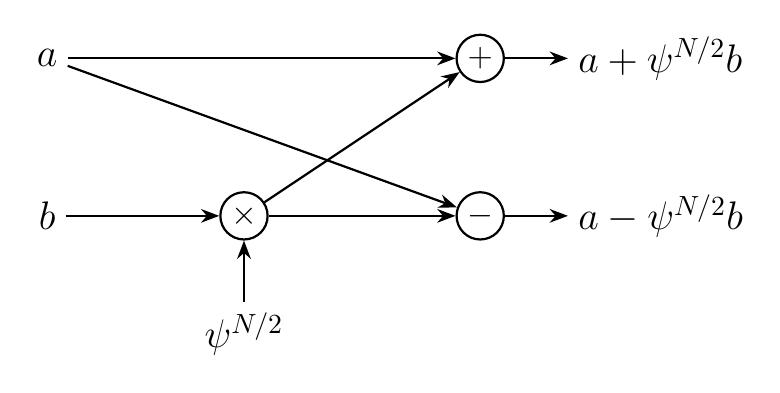
\begin{tikzpicture}[
    >=Stealth, 
    node distance=1.5cm, 
    thick,
    op/.style={circle, draw, minimum size=0.6cm, inner sep=0pt, font=\large}
]

    % --- Nós de Entrada ---
    \node (a) at (0, 2) {\Large $a$};
    \node (b) at (0, 0) {\Large $b$};

    % --- Operadores ---
    % Multiplicador (na linha de baixo)
    \node[op] (times) at (2.5, 0) {$\times$};
    
    % Somador (na linha de cima)
    \node[op] (plus) at (5.5, 2) {$+$};
    
    % Subtrator (na linha de baixo)
    \node[op] (minus) at (5.5, 0) {$-$};

    % --- Fator de Rotação (Twiddle Factor) ---
    % Entrada vindo de baixo para o multiplicador
    \node (psi) at (2.5, -1.5) {\Large $\psi^{N/2}$};
    \draw[->] (psi) -- (times);

    % --- Conexões ---
    % Linha superior (a)
    \draw[->] (a) -- (plus);          % a -> +
    \draw[->] (a) -- (minus);         % a -> - (diagonal descendo)

    % Linha inferior (b)
    \draw[->] (b) -- (times);         % b -> x
    \draw[->] (times) -- (minus);     % xb -> -
    \draw[->] (times) -- (plus);      % xb -> + (diagonal subindo)

    % --- Saídas ---
    \node[right=0.8cm of plus] (out_top) {\Large $a + \psi^{N/2} b$};
    \node[right=0.8cm of minus] (out_bot) {\Large $a - \psi^{N/2} b$};

    \draw[->] (plus) -- (out_top);
    \draw[->] (minus) -- (out_bot);

\end{tikzpicture}
\end{document}